\ProvidesFile{ap-figures.tex}[2025-01-16 figures appendix]

\begin{VerbatimOut}{z.out}
\chapter{FIGURES}
\end{VerbatimOut}

\MyIO


\begin{VerbatimOut}{z.out}

The
\verb+h+
specifier used in all the examples below
tells \LaTeX\ to put the figure
``here''
instead of trying
to find a good spot
at the top or bottom of a page.
Specifiers can be combined,
for example,
``\verb+\begin{figure}[htbp!]+''.
\end{VerbatimOut}

\MyIO


\begin{VerbatimOut}{z.out}

The complete list of figure placement specifiers:
\vspace*{6pt}
\begin{center}
  \begin{tabular}{@{}ll@{}}
    \toprule
    \bf Specifier& \bf Description\\
    \midrule
    \noalign{\vspace*{2pt}}
    \tt b& bottom of page\\
    \tt h& follow formatting rules and put here on page\\
    \tt p& on separate page of figures\\
    \tt t& top of page\\
    \tt !& try hard to put figure as early as possible\\
    \tt H& suspend formatting rules and put right here---requires \tt\char'134 usepackage\char'173 float\char'175\\
    \bottomrule
  \end{tabular}
\end{center}
\index{figure!placement specifiers (\verb+b+, \verb+h+, \verb+p+, \verb+t+, {\tt\char'041}, \verb+H+)}
\index{\verb+\begin{tabular}+}
\end{VerbatimOut}

\MyIO


% !!!! Label ``fi:not-centered'' is ``\ref{fi:not-centered}''.
% !!!! Label ``sf:four-parts-c'' is ``\ref{sf:four-parts-c}''.

\begin{VerbatimOut}{z.out}

% MyRepeat is defined in MyRepeat.sty.
\MyRepeat{This is the first paragraph.  }{5}
\end{VerbatimOut}

\MyIO


\begin{VerbatimOut}{z.out}

\begin{figure}[h]
  This is the figure.
  \caption{%
    Allocation to Common Edge for
    \(p(x_i) = 1-e^{-x_iz}\)% \frac{-x_i}z}\)%
  }
\end{figure}
\end{VerbatimOut}

\MyIO


\begin{VerbatimOut}{z.out}

\begin{sidewaysfigure}[ht]
  \setbox0=\hbox{%
    \noindent
    This is the second figure in this appendix.
    This is the second figure in this appendix.
    This is%
  }
  \dimen0=\wd0
  \hbox to \textwidth{\hss\box0\hss}
  \textwidth=\dimen0
  \advance\textwidth by 1truein
  \caption{%
    This is the caption for the second figure.
    This is the caption for the second figure.
    This is the caption for the second figure.%
  }
\end{sidewaysfigure}
\end{VerbatimOut}

\MyIO


\begin{VerbatimOut}{z.out}

\begin{sidewaysfigure}[ht]
  \setbox0=\hbox{\noindent 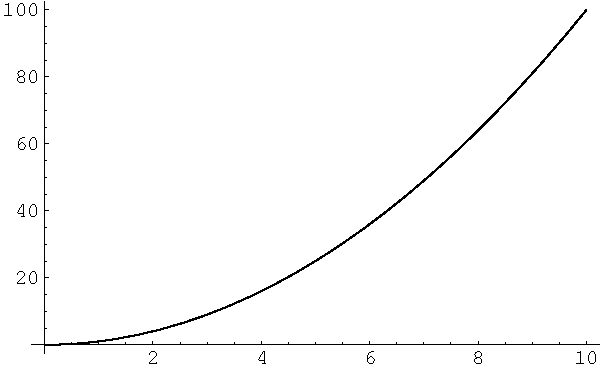
\includegraphics[width=8truein]{gr-plot.pdf}}
  \dimen0=\wd0
  \hbox to \textwidth{\hss\box0\hss}
  \textwidth=\dimen0
  \advance\textwidth by 1truein
  \caption{
    This is the caption for the third figure.
    This is the caption for the third figure.
    This is the caption for the third figure.%
  }
\end{sidewaysfigure}
\end{VerbatimOut}

\MyIO


\begin{VerbatimOut}{z.out}

\begin{figure}[ht]
  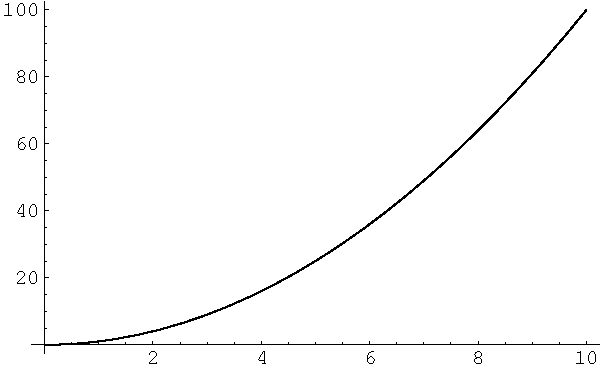
\includegraphics{gr-plot.pdf}
  \caption
  {%
    By default figures are not centered.
    This is a long caption to demonstrate that captions are single spaced.
    This is a long caption to demonstrate that captions are single spaced.%
  }
  \label{fi:not-centered}
\end{figure}
\end{VerbatimOut}

\MyIO


\begin{VerbatimOut}{z.out}

\MyRepeat{This is the second paragraph.  }{10}
\end{VerbatimOut}

\MyIO


\begin{VerbatimOut}{z.out}

\begin{figure}[ht]
  \centering
  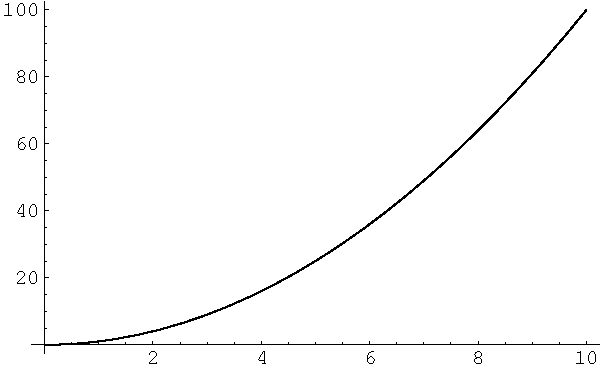
\includegraphics{gr-plot.pdf}
  \caption{Use {\tt \char'134centering\/} to center figures.}
  \label{fi:centered}
\end{figure}
\end{VerbatimOut}

\MyIO


\begin{VerbatimOut}{z.out}

\MyRepeat{This is the third paragraph.  }{15}
\end{VerbatimOut}

\MyIO


\begin{VerbatimOut}{z.out}

\begin{figure}[ht]
  \centering
  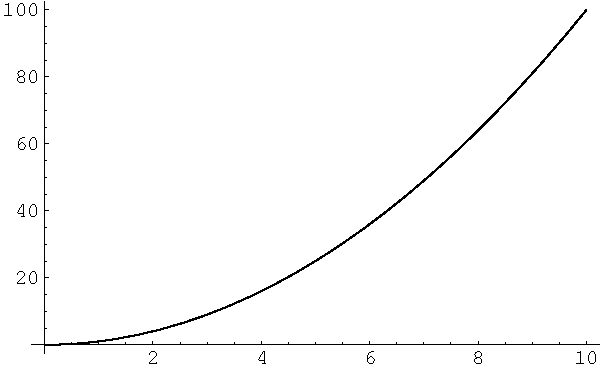
\includegraphics{gr-plot.pdf}
  \caption{This is another figuure.}
  \label{fi:another}
\end{figure}
\end{VerbatimOut}

\MyIO


\begin{VerbatimOut}{z.out}

\MyRepeat{This is the fourth paragraph.  }{10}
\end{VerbatimOut}

\MyIO


\begin{VerbatimOut}{z.out}
  
% See pages 4--5 of
%   http://mirrors.ibiblio.org/CTAN/macros/latex/contrib/caption/subcaption.pdf
% for how to use \subcaptionbox.
\begin{figure}[ht]
  % Center the entire figure (containing the two subfigures).
  \centering 
    % The \subcaptionbox for the first subfigure.
    \subcaptionbox
      % The first subcaption with a \label.
      % Use \ref{sf:two-parts-a} to print the subcaption number.
      {First subcaption.\label{sf:two-parts-a}}%
      % The first subfigure is this wide.
      [2in]%
      % This is the first subfigure.
      % You'll usually use an \includegraphics{filename}
      % inside the braces on the next line.
      {\bfseries First subfigure.}%
    % Put 0.5 inches of blank space between the subfigures.
    \hskip 0.5truein
    \subcaptionbox
      {Second subcaption.\label{sf:two-parts-b}}%
      [2in]%
      {\bfseries Second subfigure.}%
    % The caption for the entire figure (containing two subfigures).
    \caption{This figure has two subfigures arranged horizontally.}
    % The label for the entire figure.
    \label{fi:two-horizontal-parts}
\end{figure}
\ix{figure!subfigures!\(\text{1 row} \times \text{2 columns}\)}
\end{VerbatimOut}

\label{pa:subfigures}

\MyIO


\begin{VerbatimOut}{z.out}

\MyRepeat{This is the fifth paragraph.  }{10}
\end{VerbatimOut}

\MyIO


\begin{VerbatimOut}{z.out}

% See pages 4--5 of
%   http://mirrors.ibiblio.org/CTAN/macros/latex/contrib/caption/subcaption.pdf
% for how to use \subcaptionbox.
\begin{figure}[ht]
  % Center the entire figure (containing the two subfigures).
  \centering
    % The \subcaptionbox for the first subfigure.
    \vbox{\subcaptionbox  % use \vbox to stack subcaption boxes vertically
      % The first subcaption with a \label.
      % Use \ref{sf:two-vertical-parts-a} to print the subcaption number.
      {First subcaption.\label{sf:two-vertical-parts-a}}
      [2in]%
      {\bfseries First subfigure.}}%
    % Put \baselineskip blank space between the subfigures.
    \vspace*{\baselineskip}
    % The \subcaptionbox for the second subfigure.
    \vbox{\subcaptionbox  % use \vbox to stack subcaption boxes vertically
      {Second subcaption.\label{sf:two-vertical-parts-b}}
      [2in]%
      {\bfseries Second subfigure.}}%
  \caption{This figure has two subfigures arranged vertically.}
  \label{fi:two-vertical-parts}
\end{figure}
\ix{figure!subfigures!\(\text{2 rows} \times \text{1 column}\)}
\end{VerbatimOut}

\MyIO


\begin{VerbatimOut}{z.out}

\MyRepeat{This is the sixth paragraph.  }{10}
\end{VerbatimOut}

\MyIO


\begin{VerbatimOut}{z.out}
  
% See pages 4--5 of
%   http://mirrors.ibiblio.org/CTAN/macros/latex/contrib/caption/subcaption.pdf
% for how to use \subcaptionbox.
\begin{figure}[ht]
  \centering
    \subcaptionbox
      {First subcaption.\label{sf:four-parts-a}}
      [2in]%
      {\bfseries First subfigure.}%
    \hskip 0.5truein
    \subcaptionbox
      {Second subcaption.\label{sf:four-parts-b}}
      [2in]%
      {\bfseries Second subfigure.}%
    \vspace*{\baselineskip}
    \subcaptionbox
      {Third subcaption.\label{sf:four-parts-c}}
      [2in]%
      {\bfseries Third subfigure.}%
    \hskip 0.5truein
    \subcaptionbox
      {Fourth subcaption.\label{sf:four-parts-d}}
      [2in]%
      {\bfseries Fourth subfigure.}%
  \caption{This figure has four parts.}
  \label{fi:four-parts}
\end{figure}
\ix{figure!subfigures!\(\text{2 rows} \times \text{2 columns}\)}
\end{VerbatimOut}

\MyIO


\begin{VerbatimOut}{z.out}

\MyRepeat{This is the seventh paragraph.  }{10}
\end{VerbatimOut}

\MyIO


\begin{VerbatimOut}{z.out}

\newpage

\begin{figure}[ht]
  \centering 
    % Use a 5" font.
    {\fontsize{5in}{5in}\selectfont\(\hspace*{-0.07em}\sqrt 2\)}
    \caption{%
      A big ``\(\sqrt 2\)''.
      \LaTeX\ can make output big enough for T-shirts or posters.
      Square roots are printed with space before them,
      I put some negative horizontal space before this one to center it.%
    }
\end{figure}
\ix{figure!\(\sqrt 2\)}
\end{VerbatimOut}

\MyIO

\UndefineShortVerb{\|}  % so "|" in not a special character
\ix{subfigure|see{figure, subfigures}}
\DefineShortVerb{\|}  % so "|verbatim|" will be verbatim


\begin{figure}
  This is the figure.
  \caption{%
    Allocation to Common Edge for
    \(p(x_i) = 1-e^{-x_iz}\)% \frac{-x_i}z}\)%
  }
\end{figure}

\begin{VerbatimOut}{z.out}

\newpage

The remainder of this file tests having lots of figures.
There are 20 figures in this test.

\begin{figure}[ht]
  \centering
  
\includegraphics[scale=0.5]{gr-metapost-tally-01.pdf}
  \caption{Test figure 1 of 20.}
  \label{fi:1of20}
\end{figure}

\begin{figure}[ht]
  \centering
  
\includegraphics[scale=0.5]{gr-metapost-tally-02.pdf}
  \caption{Test figure 2 of 20.}
  \label{fi:2of20}
\end{figure}

\begin{figure}[ht]
  \centering
  
\includegraphics[scale=0.5]{gr-metapost-tally-03.pdf}
  \caption{Test figure 3 of 20.}
  \label{fi:3of20}
\end{figure}

\begin{figure}[ht]
  \centering
  
\includegraphics[scale=0.5]{gr-metapost-tally-04.pdf}
  \caption{Test figure 4 of 20.}
  \label{fi:4of20}
\end{figure}

\begin{figure}[ht]
  \centering
  
\includegraphics[scale=0.5]{gr-metapost-tally-05.pdf}
  \caption{Test figure 5 of 20.}
  \label{fi:5of20}
\end{figure}

\begin{figure}[ht]
  \centering
  
\includegraphics[scale=0.5]{gr-metapost-tally-06.pdf}
  \caption{Test figure 6 of 20.}
  \label{fi:6of20}
\end{figure}

\begin{figure}[ht]
  \centering
  
\includegraphics[scale=0.5]{gr-metapost-tally-07.pdf}
  \caption{Test figure 7 of 20.}
  \label{fi:7of20centered7}
\end{figure}

\begin{figure}[ht]
  \centering
  
\includegraphics[scale=0.5]{gr-metapost-tally-08.pdf}
  \caption{Test figure 8 of 20.}
  \label{fi:8of20}
\end{figure}

\begin{figure}[ht]
  \centering
  
\includegraphics[scale=0.5]{gr-metapost-tally-09.pdf}
  \caption{Test figure 9 of 20.}
  \label{fi:9of20}
\end{figure}

\begin{figure}[ht]
  \centering
  
\includegraphics[scale=0.5]{gr-metapost-tally-10.pdf}
  \caption{Test figure 10 of 20.}
  \label{fi:10of20}
\end{figure}

\begin{figure}[ht]
  \centering
  
\includegraphics[scale=0.5]{gr-metapost-tally-11.pdf}
  \caption{Test figure 11 of 20.}
  \label{fi:11of20}
\end{figure}

\begin{figure}[ht]
  \centering
  
\includegraphics[scale=0.5]{gr-metapost-tally-12.pdf}
  \caption{Test figure 12 of 20.}
  \label{fi:12of20}
\end{figure}

\begin{figure}[ht]
  \centering
  
\includegraphics[scale=0.5]{gr-metapost-tally-13.pdf}
  \caption{Test figure 13 of 20.}
  \label{fi:13of20}
\end{figure}

\begin{figure}[ht]
  \centering
  
\includegraphics[scale=0.5]{gr-metapost-tally-14.pdf}
  \caption{Test figure 14 of 20.}
  \label{fi:14of20}
\end{figure}

\begin{figure}[ht]
  \centering
  
\includegraphics[scale=0.5]{gr-metapost-tally-15.pdf}
  \caption{Test figure 15 of 20.}
  \label{fi:15of20}
\end{figure}

\begin{figure}[ht]
  \centering
  
\includegraphics[scale=0.5]{gr-metapost-tally-16.pdf}
  \caption{Test figure 16 of 20.}
  \label{fi:16of20}
\end{figure}

\begin{figure}[ht]
  \centering
  
\includegraphics[scale=0.5]{gr-metapost-tally-17.pdf}
  \caption{Test figure 17 of 20.}
  \label{fi:17of20}
\end{figure}

\begin{figure}[ht]
  \centering
  
\includegraphics[scale=0.5]{gr-metapost-tally-18.pdf}
  \caption{Test figure 18 of 20.}
  \label{fi:18of20}
\end{figure}

\begin{figure}[ht]
  \centering
  
\includegraphics[scale=0.5]{gr-metapost-tally-19.pdf}
  \caption{Test figure 19 of 20.}
  \label{fi:19of20}
\end{figure}

\begin{figure}[ht]
  \centering
  
\includegraphics[scale=0.5]{gr-metapost-tally-20.pdf}
  \caption{Test figure 20 of 20.}
  \label{fi:20of20}
\end{figure}
\end{VerbatimOut}

\MyIO
